\chapter{Background\label{background}}

JavaScript is one of the primary languages in programming web technologies. It can interact with the document's object model (DOM) and provides different impressive functionality. Because of these features, JavaScript is extensively used on nearly every website, and all of the browsers allow JavaScript, as it helps in making the page dynamic and it keeps a user engaged. 

JavaScript's capability of interacting with the DOM also grants it with the potential of injecting malicious code in the script dynamically. There has been various flavors and types of malicious JavaScript, and one of the most wicked ones is cross-site scripting (XSS).

\section{Cross site scripting (XSS)}

An XSS attack targets websites that do not verify and sanitize user input in a proper way; that enables attackers to inject malicious code into the web page. An attacker may insert a link to the third party malicious website into the benign web page. If a user visits such an infected page and clicks the link, the link will take the user to the malicious website and steal the user's cookies and other sensitive information stored in the browser. An attacker can use this information to impersonate that user. Attackers can also employ various kind of obfuscation technique to conceal the exploit in the link and makes it resemble like a legitimate link. There are commonly three types of XSS attacks: stored XSS, reflected XSS and DOM-based XSS ~\cite{g12}. 

\subsection{Stored Cross Site Scripting}

Stored cross-site scripting targets the websites that store the user input first in databases or the file system and later reflect the user input to the web pages. If the input has not been sanitized or encoded and the data contains an attack, it will inject the attack in the web pages. This type of attack affects multiple users of the website ~\cite{g12}.

Stored cross site scripting attack. Attacker is storing malicious script to database using a form. The data is stored to database without proper input validation and and reflected to the web page without output validation. A user clicks on the malicious link and the attacker hijacks the information stored in user?s browser.

\begin{figure}[htb]
\centering
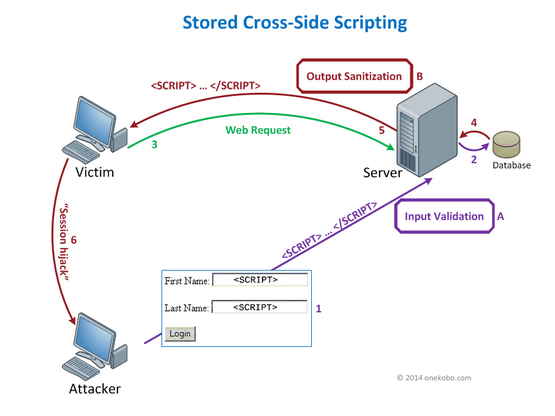
\includegraphics[width=1.0\textwidth]{image/sxss.png}
\caption[Stored cross-site scripting attack]{Stored cross-site scripting attack ~\cite{g14}} 
\label{fig:sxss}
\end{figure}

\subsection{Reflected cross-site scripting}

Reflected cross-site scripting targets the websites that reflect a user's input immediately to the web page. If not encoded, it may allow an attacker to inject malicious code into the dynamic webpage. However, an attacker can only change his web page result, though the attacker can persuade a user to click on a link, which can lead that user to a malicious website ~\cite{g13}.


Reflected cross site scripting attack. An attacker identifies a vulnerable website and inject malicious link. The attacker then convinces the user to click on the link using social engineering. The user clicks on the link and becomes victim of reflected XSS attack. 


\begin{figure}[htb]
\centering
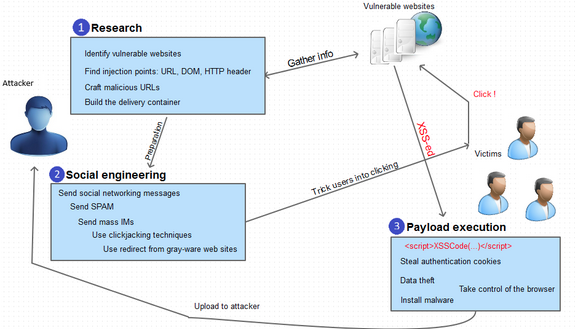
\includegraphics[width=15cm,height=15cm,keepaspectratio]{image/rxss.png}
\caption[Reflected cross-site scripting attack]{Reflected cross-site scripting attack ~\cite{g13}} 
\label{fig:rxss}
\end{figure}

\newpage

\subsection{DOM based XSS Attack}

Every HTML page has an associated document object model (DOM) that consists of the HTML page objects. These objects represent the document properties. When a JavaScript within an HTML page executed, the browser provides the DOM of the HTML page to the script. A JavaScript can interact with the DOM and may perform an action based on the properties of the objects in DOM to make the page more interactive and dynamic. A DOM XSS attack targets the improper treatment of the data from its associated DOM in the HTML pages ~\cite{g20}.

{\bf An example of DOM based XSS attack.}

\begin{figure}[htb]
\centering
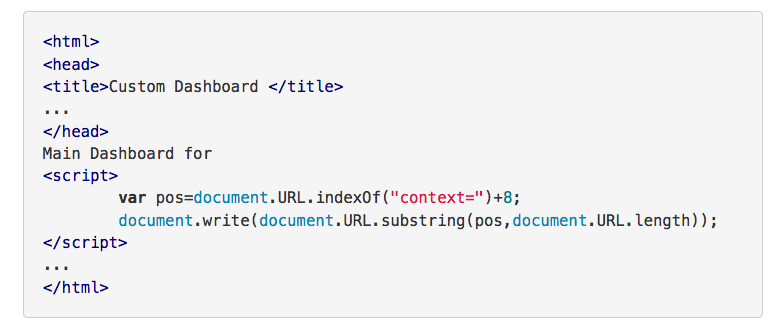
\includegraphics[width=15cm,height=15cm,keepaspectratio]{image/dxss.png}
\caption[DOM based cross-site scripting attack]{In this html page, JavaScript variable pos is set to the value of context field form the URL ~\cite{g20}} 
\label{fig:dxss}
\end{figure}

\begin{figure}[htb]
\centering
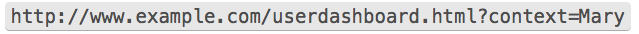
\includegraphics[width=15cm,height=15cm,keepaspectratio]{image/dxss2.png}
\caption[DOM based cross-site scripting attack example ]{: User click on this URL which sets the variable pos to value of context i.e. Mary ~\cite{g20}} 
\label{fig:dxss2}
\end{figure}

\newpage

{\bf Example of the same URL with embedded malicious script.}

\bigskip

\begin{figure}[htb]
\centering
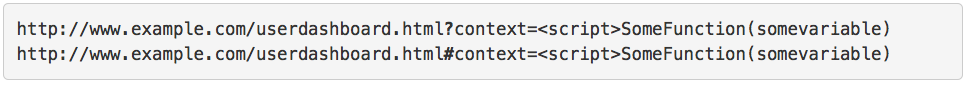
\includegraphics[width=16cm,height=20cm,keepaspectratio]{image/dxss3.png}
\caption[DOM based cross-site scripting attack example]{An attacker embeds a malicious script as value of context field ~\cite{g20}} 
\label{fig:dxss3}
\end{figure}

The user clicks on the above URL, which sends the request with the context value as malicious JavaScript. The browser builds the DOM of the web page after receiving the response from the server and sets the value of the property document.url to the value of the context. When the script gets executed it updates the raw HTML of the page with the malicious script and the malicious script now gets carried out by the browser resulting in the attack.

\bigskip

\begin{figure}[htb]
\centering
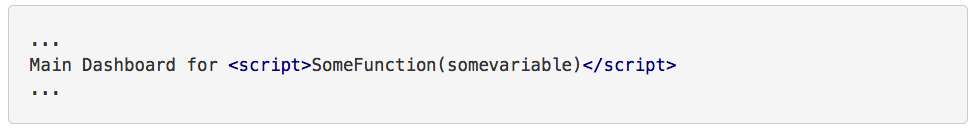
\includegraphics[width=16cm,height=20cm,keepaspectratio]{image/dxss4.png}
\caption[HTML page with embedded malicious JavaScript]{HTML page with embedded malicious JavaScript ~\cite{g20}} 
\label{fig:dxss4}
\end{figure}

\bigskip

\section{Other variants of JavaScript Attack}

Cross-site request forgery is also a standard JavaScript attack and has been listed as number five in the Top 10 web applications security risks by OWSAP 2013[2]. Cross-site request forgery refers to sending malicious requests to an authorized user of websites that websites trusts. In cross-site request forgery, an attacker attempts to send a state change request such as a fund transfer or an email change. An attacker convinces an authorized user to execute unauthorized commands by use of social engineering tricks such as sending an email that looks authorized to the user. By clicking on the link may submit that forged request if the user is already login to the website. A website has no way to know if the request is a legitimate one or a forged one as a website stored the login credentials and other sensitive information of the user in the cookies or session in the browser. That is why this attack is also known as session over-riding attack.

{\bf A legitimate request example:}


{\bf Alice wants to transfer funds to Bob' account.}

\bigskip

\begin{figure}[htb]
\centering
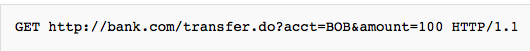
\includegraphics[width=16cm,height=20cm,keepaspectratio]{image/csrf1.png}
\caption[Cross-site request frogery attack]{A legitimate fund transfer request to transfer money to Bob's account using GET request ~\cite{g20}} 
\label{fig:csrf1}
\end{figure}

\bigskip

{\bf A malicious request}

The attacker can change the value in GET request so that it transfers the fund to the attacker's account and tricks the victim using social engineering to click on the below link to transfer money to his account.
The below forged requests can be by sent an email or can be injected in a website the user is most likely to visit while transferring funds.
\bigskip

\begin{figure}[htb]
\centering
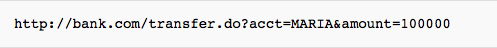
\includegraphics[width=16cm,height=20cm,keepaspectratio]{image/csrf2.png}
\caption[Malicious request forged by the attacker]{Malicious request forged by the attacker. Here name value is changed to MARIA form BOB and amount value is changed to 100000 form 100} 
\label{fig:csrf2}
\end{figure}

\section{Security measures adopted to prevent malicious JavaScript Attack}

To avoid an attack, the following actions can be taken: escape and sanitize all the users input data, whitelist input validation, and employ content security policy using sandboxing. Modern web browsers are taking the following measures to prevent or restrain a JavaScript attack: sandboxing and the same origin policy [5]. Sandboxing limits the scope of a script, preventing the attacks from spreading system wide. The same origin policy prevents a script from one source to access resources from a different origin. However, attackers leverage the flaws in the websites and insecure practices and allowing them to circumvent the above two restrictions. The common defects and unsafe practices used by the attackers are vulnerable JavaScript inclusion and insecure JavaScript generation [15]. JavaScript inclusion injects the third domain JavaScript by using the src attribute of a script tag in the top level document and thus defy the purpose of same origin policy [15]. Attackers use eval() function for dynamic generation of malicious JavaScript code. According to research by [15], 66.4\% of the website uses the insecure practice of JavaScript inclusion, and 74.9\% uses dynamic JavaScript generation.

Modern approaches are using machine learning technology in combination with de-obfuscation/emulation for better performance and accuracy [1]. Machine learning can be used in analyzing and capturing the structural information of a malicious JavaScript program by extracting the abstract syntax tree, while emulation can be used to analyze the behavior of a malicious JavaScript program. Obtaining structural information for analysis is known as static analysis while using emulation to execute the exploit to examine and analyze the behavior and impact of an exploit is known as dynamic analysis. According to TARDIS [1], dynamic analysis tends to be more accurate than static analysis, but it has more performance overhead.  

\section{Static Analysis}

Static analysis analyzes source code without executing it, and is commonly used as a technique for troubleshooting a computer program [15]. Static analysis helps in understanding the composition of a program. The static analysis aims at examining the correctness and consistency of presentation and description of a software application, and serves as the first step in software quality control procedure [14]. It can be performed automatically using specific tools such as parsers, data flow analyzers, syntax analyzers, etc. Static analysis can also be followed by dynamic analysis for uncovering the subtle defects or vulnerabilities. Static and dynamic analysis together refers as glass box testing.

TARDIS is based on purely static analysis of malicious and benign JavaScript, and combines static analysis with SLM for robust feature extractions. In our project, we are using static analysis for analyzing the program syntax, and a JavaScript parser for capturing the abstract syntax tree, and examining the structure and usage of individual JavaScript statements, keywords, and reserved words. We are performing automatic static analysis by parsing the scripts in the program. A more detailed description of TARDIS is available in section 2.7. 

\section{Dynamic Analysis} \label{dynamic_analysis}

Dynamic analysis involves examining source code by execution. It analyzes the action, impact, and behavior of software before and after the execution of the software in a controlled manner and environment. The execution of software can be carried out in either artificial or real application environment. Path testing and branch testing are two primary dynamic analysis techniques. Branch testing aims at traversing every branch of a program at least once while path testing attempts to exercise as many logical paths as possible.

Dynamic analysis and detection of a JavaScript exploit require a detection system that can observe and examine the execution of a JavaScript code during run-time. To capture this information, a JavaScript program is either executed in a sandbox environment or the detection system interacts with the JavaScript engine of the web browser. The detection system monitors and tracks the flow of the execution events, which result in modifications to the environment state.

\section{Related Work} \label{related_work}

This section presents the recently advanced approaches in detecting and analyzing malicious JavaScript using machine learning technology. These approaches are either using static analysis, dynamic analysis or a combination of both.

\subsection{JStill (Mostly Static Approach) ~\cite{g6}} \label{jstill}

The JStill approach is mostly static. However, in conjunction with static analysis, JStill uses a lightweight runtime inspection, which helps in analyzing the essential characteristics of an obfuscated malicious program. JStill performs static analysis to capture the characteristics of an exploit. However, a static analysis alone may not be accurate due to the obscured nature of the malicious program. An obfuscated malicious program has to be de-obfuscated before fulfilling its malicious intent and requires particular function invocations. JStill leverages this observation of function invocation to inspect the runtime behavior of obfuscated code. JStill examines the function invocation pattern by a malicious program using the browser's runtime operations and hence does not incur any extra performance overhead of dynamic analysis that requires executing an exploit in a controlled environment.  JStill can be implemented in a browser. The average performance overhead of JStill is 4.9\%. It shows higher performance overhead i.e. > 8\% for yahoo.com and sina.com.cn. JStill also tends to give a higher false positive rate for a benign obfuscated JavaScript program.

\subsection{Zozzle: Fast and Precise In-Browser JavaScript Malware Detection ~\cite{g24}} \label{zozzle}

Zozzle is a combination of both static and dynamic analysis. Zozzle mostly uses static analysis for better performance and high throughput. It also uses a component of dynamic analysis for better accuracy and the analysis of an obfuscated malicious JavaScript program. Static analysis of Zozzle uses Bayesian classification of hierarchical features of the JavaScript abstract syntax tree to extract the essential predictive features and quick scanning. To handle the obfuscation, Zozzle uses a small runtime component. This component extracts and processes the JavaScript that is generated at runtime using \texttt{eval()}, \texttt{document.write()}, etc. It then sends this runtime generated code to its static analyzer right before the execution. Zozzle has a very high throughput as big as one megabyte of JavaScript code per second and an exceptionally low false positive rate of 0.0003\%. 

\subsection{Cujo: efficient detection and prevention of drive-by-download attacks ~\cite{g23}} \label{cujo}

Cujo combined both static analysis and dynamic analysis for automatic detection and blocking of drive-by download attacks. Static analysis extracts lexical tokens representing reserved words, literals, and identifiers. The dynamic analysis uses a lightweight sandboxing environment that analyzes execution behaviors. Both the static and dynamic features are explained further using machine learning technique for robust detection of an exploit. Cujo can be embedded in a web proxy, and it tends to reach a very high accuracy of 94\% in detecting an attack with a very low false positive rate. Cujo is a learning-based detection tool and uses the support vector machine learning algorithm. In spite of high precision, the dynamic analysis part of Cujo incurs performance overhead and the run time of Cujo is 500 ms per web page.

\subsection{IceShield: Detection and Mitigation of Malicious Websites with a Frozen DOM ~\cite{g25}} \label{iceShield}

IceShield performs in browser dynamic analysis and de-obfuscation to detect and mitigate a malicious JavaScript attack. IceShield is entirely based on dynamic analysis. It de-obfuscates the code first and then performs analysis on an exploit presented in clear text after deobfuscation. IceShield primarily targets the types of attack that compromise the DOM and injects malicious code. IceShield makes use of a heuristic approach to discover an attacker from a benign user visiting and accessing the web page. IceShield is capable of detecting the part of the internet page that is malicious and modifies the page accordingly to block the attack. It is entirely implemented in JavaScript, and hence lightweight. It is also independent of a browser and can be applied in embedded browsers such as smartphone browsers. IceShield detection accuracy is 98\%, and performance overhead is 12ms for a website and 80 ms for a smartphone.

\subsection{EarlyBird: Early Detection of Malicious Behavior in JavaScript Code ~\cite{g25}}

EarlyBird uses dynamic analysis to perform dynamic, efficient detection of an exploit. A dynamic analysis requires execution of an exploit which may also result in potential damage to the underlying system. EarlyBird attempts to prevent the severity of harm caused by the execution of a malicious script by detecting it in on early phase of execution. It uses a set of predefined events and JavaScript execution results in particular sequences of these events. These event tracking can be used for various features extractions. This sequence of events is then mapped to vector space and uses linear support vector machine algorithm for learning and detection to achieve better protection of the underlying system. EarlyBird restricts the amount of exploit code that gets executed by a factor of 2. EarlyBird makes use of support vector machine and can achieve a good performance of 93\% with very low false positive. 

\subsection{Wepawet ~\cite{g8}} \label{wepawet }

Wepawet uses an emulation techniques and combines it with anomaly detection for automatic identification of a drive-by download attack. Wepawet supplies the features of regular JavaScript to the machine learning classifier and uses emulation to detect the behavior of malicious anomalous JavaScript by analyzing it against previously verified features. Wepawet achieves a low false negative rate and no false positives on the data set tested.

\subsection{PJScan: Static Detection of Malicious JavaScript-Bearing PDF Documents ~\cite{g4}}

A pdf document is a commonly used file format, and they provide many features. Attackers have discovered a way to hide malicious scripts inside PDF files. PJScan uses static analysis on extracted JavaScript code to detect the JavaScript-bearing malicious PDF documents. PJScan incurs a significant low run-time overhead as compared to other previous work done that uses dynamic analysis approaches. PJScan can work efficiently on both known and unknown malicious JavaScript. PJScan utilized a lexical analysis approach and machine learning technology for automatic construction of the models, which can then be used to detect a pdf attack. 

\subsection{Prophiler: A Fast Filter for the Large-Scale Detection of Malicious Web Pages ~\cite{g16}}

Prophiler uses static analysis for rapid detection of the presence of an exploit in a web page. Prophiler uses a JavaScript program to extract significant features from HTML content of a webpage. These features are then supplied to a machine learning technology. The primary purpose of Prophiler is to reduce the resources and cost of dynamic analysis tools for detection and analysis of a drive-by download attack.  Dynamic analysis tools are capable of detecting a drive-by download attack precisely, but they have costly analysis methods usually in the order of tens of seconds per page. This overhead is generally too costly for performing analysis on an extensive set of web pages. Prophiler is effective in reducing the load of dynamic analysis tools by 85\%, but it still incurred 270 ms per page and has a 13.7\% false positive rate.

Dynamic analysis provides better accuracy in detecting an exploit as compared to static analysis, but it incurs a performance overhead. Static analysis is faster than dynamic analysis, but not capable of detecting obfuscated malicious JavaScript efficiently. After examining the recent works done towards the detection of malicious JavaScript, we discover that most of the works are taking advantage of both approaches. They are trying to be mostly static to achieve the desired speed and implementing a lightweight dynamic analysis component for effectiveness without sacrificing performance.

\newpage

\bigskip

A snapshot of a benign JavaScript program

\bigskip

\begin{figure}[htb]
\centering
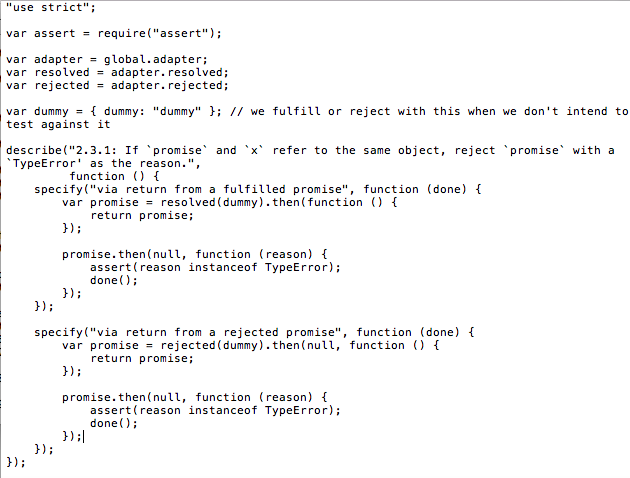
\includegraphics[width=15cm,height=25cm,keepaspectratio]{image/benign.png}
\caption[Benign script sample]{A sample of malicious script form test data set} 
\label{fig:benign}
\end{figure}

\newpage

\bigskip

A snapshot of a malicious JavaScript program

\bigskip

\begin{figure}[htb]
\centering
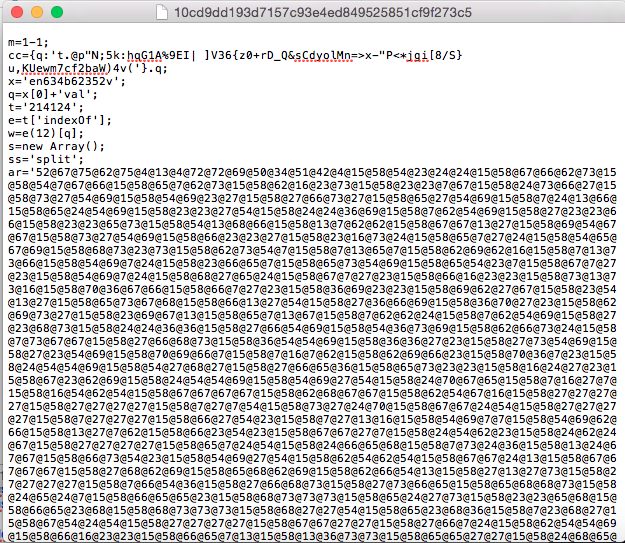
\includegraphics[width=15cm,height=35cm,keepaspectratio]{image/malicious.png}
\caption[Malicious script sample]{A sample of malicious script form test data set} 
\label{fig:malicious}
\end{figure}

\newpage

\bigskip

A snapshot of a obfuscated JavaScript program

\bigskip

\begin{figure}[htb]
\centering
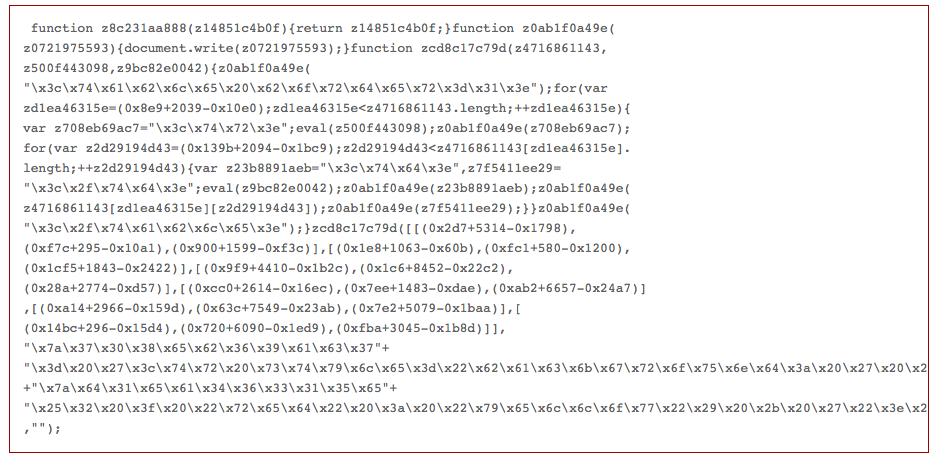
\includegraphics[width=16cm,height=25cm,keepaspectratio]{image/obfuscated.png}
\caption[Obfuscated script sample]{A sample of obfuscated script form test data set} 
\label{fig:obfuscated}
\end{figure}

\newpage

\section{TARDIS} \label{tardis}

TARDIS (Towards Robust Detection of Malicious JavaScript) ~\cite{g1} developed by Professor E J Jung et al. at the University of San Francisco, is a completely static analysis tool. It only requires the source code of the exploit and hence does not require execution and thus avoids dynamic analysis performance overhead. Text based static analysis is not very useful in detecting obfuscated code as static analysis approaches tend to have a high false positive rate on minified, obfuscated benign scripts. To achieve optimal accuracy TARDIS has been supplemented with a powerful Statistical Language Model.

TARDIS's static analysis focuses that can differentiate between malicious and benign scripts based on their textual attributes. Analyzing textual attributes is purely static and does not require the execution of the source code. Some example of these textual attributes can be the use of whitespace, line breaks, the length of sentences, comments in a benign and malicious script, and the use of various keywords. These textual attributes can be used to discover a pattern in the way a malicious and benign JavaScript is written. These features alone are not sufficient for detecting a malicious code efficiently. An attacker may avoid detections by a slight change in their code generation algorithm, which requires analyzing more robust features incurring significant work on the part of the attacker in modifying their code generation algorithm to escape detection.

To achieve this requirement TARDIS makes use of a statistical language model for automated feature extraction by using a JavaScript parser and an abstract syntax tree in addition to the textual attributes features discussed in the previous section.

\subsection{Abstract syntax tree}

An abstract syntax tree represents the syntactic structure of a program by using nodes of a tree. An AST represents constants or variables as leaf nodes, and operators and statements as an inner node of the AST. Characteristic of an abstract syntax tree can be used to extract features that are difficult to be evaded by an attacker. Modification in the features of AST towards avoiding detection will require imitation of the AST of a benign code. A malicious code makes use of certain functions with higher frequency to carry out attacks such as string concatenation or \texttt{fromCharCode ()} etc. Concealing the detection of these features by an AST will require the attacker to use a new algorithm to generate malicious code that avoids the textual attributes detection.

\subsection{Statistical Language Modeling (SLM) ~\cite{g11}}

Statistical language modeling makes use of a statistical language model. A statistical Language model is defined as a probability distribution of a string (s) in a sentence. The probability distribution of a string (s) represents the frequency of occurrence of (s) as a sentence. The most widely used SLM techniques are N-gram models and its variants [20].

TARDIS makes use of SLM for automatic feature extraction by employing a JavaScript parser. The JavaScript parser parses benign and malicious scripts and extracts essential features. These extracted features are then used to create SLM benign and SLM malicious training model that can be used to classify a benign or a malicious script. 

\subsection{TARDIS SLM model} \label{tardis_slm}

The parser generates a collection of words based on certain delimiters after parsing a training corpus. These words then can be appended together and form an n-gram. N-gram represents a consecutive sequence of n words from a sentence. These n-grams constitute the features of the training model. The SLM training model describes the features as key-value pairs, where the key denotes a feature/n-gram and the values represents the probability of occurrence of that particular element in the model.  This mapping of n-grams with probability forms the statistical model of TARDIS's static analysis technique. This mapping can then be used to estimate the probability that a document belongs to a particular class (benign or malicious).

TARDIS generates SLM models for benign and malicious scripts. SLM benign models are computed over benign scripts while the SLM malicious models are calculated using malicious scripts. While testing both the models are used to estimate the overall probability of a document belonging to either of the models. The model that gives the higher probability wins and the testing script is classified to the winning model.

TARDIS makes use of the following formula to estimate the likelihood of categorization of a script to either the benign or the malicious category.

\subsection{N-grams SLM model} \label{n-grams}

An n-gram model can have different forms, and each of these forms can be used in generating a model. Each of these models can provide different information and as well as the features and can have a different impact on the words and probability mapping, precision of the model. TARDIS experimented with models computed based on n-grams of size 1, 2, 3, and 4 to tune the accuracy. N-grams of size 1 considers each character as a feature while n-grams of size 2 joins together two consecutive characters. Similarly, a model based on n-grams of size 3 and four can be computed.  N-grams model of size 1 tends to lose the surrounding context while n-grams model of a large size can provide too many surrounding contexts but less meaningful matches. Mostly n-grams of size 2 or 3 provide meaning full match with adequate surrounding contexts. TARDIS built its training model for n-grams of size 1 to n-grams of size 4 and compute the accuracy of each of the model in order to identify which n-grams model provides better accuracy in terms of classification. TARDIS proposes the use of three categories of n-gram model. Each of them computes the benign and malicious training model for n-gram of size 1, 2, 3, and 4. 


\subsection{Character level n-grams}

A character level n-grams model expresses the content of an input script rather than the composition of the input script. A character level n-grams model uses characters as tokens. It converts the input sequence to a collection of the characters and joins the consecutive characters to form different sizes of n-grams.

Given a sequence of input script as

\texttt"var str = "javaScript"

An n-gram of size one will look like

\texttt['v', 'a', 'r', ' ', 's', 't', 'r', '=', '"', 'j', 'a', 'v', 'a', 'S', 'c', 'r', 'i', 'p', 't', '"']

An n-gram of size three will look like

\texttt['v', 'a', 'r'], ['a', 'r', ' '], [ 'r', ' ', 's'], [' ', 's', 't'], ['s', 't', 'r'], ['t', 'r', '='], 
['r', '=', '"'], ['=', '"', 'J'], ['"', 'J', 'a'], ['a', 'v', 'a'], [''v', 'a', 's'], ['a', 'S', 'c'], ['S', 'c', 'r'], ['c', 'r', 'i'], ['r', 'i', 'p'], ['i', 'p', 't'], ['p', 't', 'i']

A character level n-grams model can successfully extract useful predictive features such as JavaScript keywords, operators, and frequency of use of increment, decrement operators, etc. However, it is not very informative regarding the structure, and semantically meaningful input sequences such as function call as a character level n-grams model break down the function call into a list of characters.

\subsection{Keyword Transformation}

Keyword transformation n-grams model reserves all the JavaScript keywords as they are and uses them without breaking down into character tokens. It treats all the other input sequence the same as character level n-grams and calculates the model for different n-gram size. TARDIS uses a list of reserved JavaScript keywords to identify the keywords in an input script. Keyword transformation also does not count space character in the model generation. 

Given a sequence of input script as

\texttt var i = 1;

Keyword transformation n-grams of size 1 will look like 

['var', 'i', '=', '1', ';']

Keyword transformation n-grams of size 3 will look like

['var', 'i', '='], ['i', '=', '1'], ['=', '1', ';']

Here 'var' is a JavaScript keyword and hence, it is used as it is without breaking down into characters.  Keyword transformation represents both the semantics and the content of a program. Keyword transformation can be used in extracting common programming language features such as variable assignments, which is helpful in classifying a benign script if it is not obfuscated ~\cite{g1}. However, it does not prove very beneficial in identifying malicious, obfuscated scripts ~\cite{g2}.

\subsection{Composite word-type transformation}

Keyword transformation is not very accurate in analyzing obfuscated JavaScript. An obfuscated JavaScript program makes use of string encoding to conceal its payload. Keyword or character level conversion on an encoded string results in a substantial number of unique characters that do not present any significant information. To manage efficient detection of obfuscated malicious JavaScript, TARDIS is uses composite word type transformation. The composite word type transformation practices a predefined class based transformation. It assigns each token to a particular class and computes the probability model by computing the frequency of appearance of these classes in the model. Representing a program based on these classes reduces randomness in a program to more significant features. Commonly a program consists of  digits, hexadecimal numbers, white spaces, punctuation, etc. Composite word type transformation provides a separate class for each type of element. Characters other than the above-defined classes are combined and interpreted as whole words. 

Composite word type transformation n-grams of size 1 of 'var i = 1;'

['var', 'SPACE', 'i',  'SPACE', 'PUNCTUATION', 'SPACE', 'DIGIT', 'PUNCTUATION']

Composite word type transformation  n-grams of size 3 of 'var i = 3 ;'

['var', 'SPACE' , 'i'],  ['SPACE' , 'i', 'SPACE'], [ 'i', 'SPACE','PUNCTUATION'], ['SPACE','PUNCTUATION','SPACE'], ['PUNCTUATION','SPACE', 'DIGIT'], ['SPACE', 'DIGIT', 'PUNCTUATION']

\section{Malicious Probability Query Strategy}

A composite word type transformation reduces randomness and uniqueness of an obfuscated JavaScript program and group together the unique characters using a predefined class.  Probability model generation of an obfuscated script requires extra control over the method by which probability of a particular type of n-gram is estimated. TARDIS introduces an alphanumeric probability strategy for computation of malicious model. An alphanumeric probability strategy calculates the probability of string consists of only alphanumeric characters based on the following formula

\[ (1/ 62) ^ n\] 

where  n is the length of the string. Here 62 is the sum of 26 upper case alphabets from A to Z, 26 lower case alphabets from a to z, and ten digits from 0 to 9.

TARDIS also performs smothering of the probability of an n-gram which is not present in the model to avoid setting the probability as zero.
